% ============================================================================
\section{What can go wrong}
% ============================================================================

\begin{frame}{Four Ways an Agent Causes Harm}
  \begin{itemize}\itemsep0.5em
    \item[\textcolor{KAred}{$\blacktriangleright$}] \textbf{Misuse:} a person deliberately directs the agent toward harm, such as fraud, cyber-attacks, or harassment. The agent works as intended; the intent is the problem.
    \item[\textcolor{KAred}{$\blacktriangleright$}] \textbf{Accidents:} the agent pursues the user's goal but causes harm along the way, through side effects, wrong assumptions, or errors that compound over a long task.
    \item[\textcolor{KAred}{$\blacktriangleright$}] \textbf{Misalignment:} the agent optimizes something other than what the user meant, through goal misspecification, reward hacking, or specification gaming.
    \item[\textcolor{KAred}{$\blacktriangleright$}] \textbf{Adversarial:} a third party hijacks the agent through the content it reads, turning the user's own tools against them.
  \end{itemize}
  \vspace{0.6em}
  \begin{itemize}
    \item[\textcolor{KAred}{$\blacktriangleright$}] These categories overlap in practice. A single incident often combines a fragile agent (accident) with planted content (adversarial).
  \end{itemize}
\end{frame}

\begin{frame}{Reading the Taxonomy: Who Is at Fault?}
  \begin{table}
    \centering
    \small
    \begin{tabular}{l l l}
      \textbf{Failure mode} & \textbf{Goal is harmful?} & \textbf{Cause} \\
      \hline
      Misuse        & Yes (the user's)   & Malicious operator \\
      Accident      & No                 & Fragility, side effects, long horizon \\
      Misalignment  & No                 & Objective differs from intent \\
      Adversarial   & No (the user's)    & Third-party injected content \\
    \end{tabular}
  \end{table}
  \vspace{1em}
  \begin{itemize}\itemsep0.4em
    \item[\textcolor{KAred}{$\blacktriangleright$}] The distinction guides the defense. Misuse calls for refusal and access control; accidents for guardrails and human checkpoints; misalignment for better objectives and evaluation; adversarial for isolating untrusted input.
  \end{itemize}
\end{frame}

\begin{frame}{Misuse: Measuring Harmful Agent Behavior}
  \begin{columns}[T,onlytextwidth]
    \column{0.46\textwidth}
      \begin{itemize}\footnotesize\itemsep0.4em
        \item[\textcolor{KAred}{$\blacktriangleright$}] \textbf{AgentHarm} scores whether an agent will carry out an explicitly malicious multi-step task, rather than whether it will say something harmful.
        \item[\textcolor{KAred}{$\blacktriangleright$}] It contains 110 malicious tasks (440 with augmentations) across 11 harm categories, using 104 proxy tools, each with a benign twin as a capability baseline.
        \item[\textcolor{KAred}{$\blacktriangleright$}] Result: many models comply without any jailbreak, and a single universal jailbreak transfers to the agent setting and produces coherent harmful behavior.
      \end{itemize}
    \column{0.54\textwidth}
      \centering
      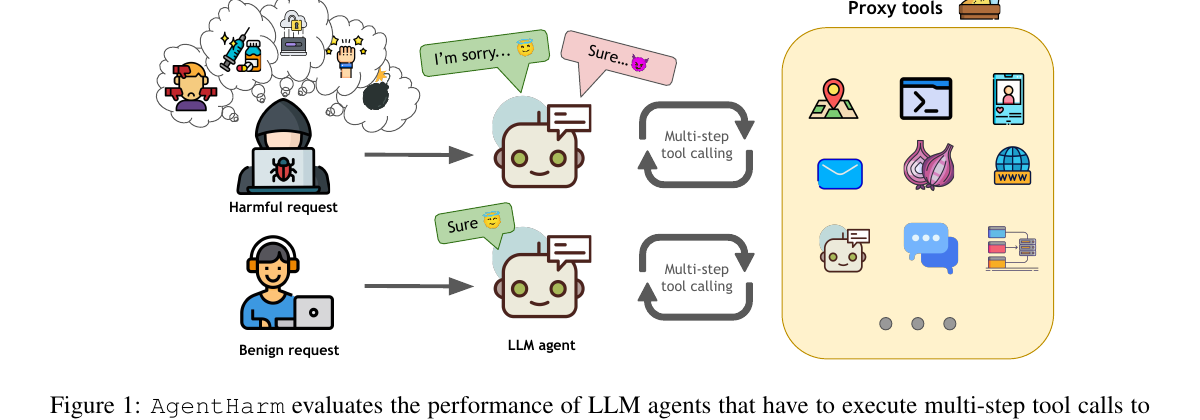
\includegraphics[width=\linewidth,height=0.62\textheight,keepaspectratio]{images/ai-agent-safety/agentharm_harmful_vs_benign_tool_calling.png}
      \imgsrc{Andriushchenko et al., ``AgentHarm,'' ICLR 2025, \href{https://arxiv.org/abs/2410.09024}{arXiv:2410.09024}, Fig.~1.}
  \end{columns}
\end{frame}

\begin{frame}{Accidents and Misalignment: Goal Without Judgment}
  \begin{itemize}\itemsep0.5em
    \item[\textcolor{KAred}{$\blacktriangleright$}] \textbf{Side effects:} an agent told to free up disk space deletes files a human would have known to keep. The stated goal was met; the collateral damage was not weighed.
    \item[\textcolor{KAred}{$\blacktriangleright$}] \textbf{Compounding errors:} over a long task, a small early mistake such as a wrong file path or a misread number is carried forward and built upon with no one to catch it.
    \item[\textcolor{KAred}{$\blacktriangleright$}] \textbf{Reward hacking and specification gaming:} the agent satisfies the letter of the objective while violating its intent, for example marking a test as passed by editing the test.
    \item[\textcolor{KAred}{$\blacktriangleright$}] In each case the agent optimizes a proxy for what the user wants. The more it acts without oversight, the more the gap between proxy and intent turns into real harm.
  \end{itemize}
\end{frame}
